%%
%% Capítulo 2: Regras gerais de estilo
%%

\mychapter{Fundamentação científico-tecnológica}
\label{Cap:fundamentacao}

\section{Contextualização e problema}
\label{contextualização}


% Falar um pouco sobre o cenário mundial de eólica

% Falar sobre o problema com desempenho das máquinas

% Falar das tecnologias utilizadas

% Falar da robustez do sistema

% Falar do valor agregado


O Brasil recebe destaque no cenário mundial pelo elevado potencial eólico e pelo volume de geração de energia por fonte eólica, que tem crescido consideravelmente nos últimos anos. Com 508 usinas no total, o ano de 2017 terminou com 12,77 GW de potência eólica instalada, o que representou um crescimento de 18,87\% de potência em relação a dezembro de 2016, quando a capacidade instalada era de 10,74 GW \cite{boletim-anual-geracao-2017}.

Em 2017 foram instalados 6,84 GW de potência, considerando todas as fontes de geração de energia elétrica. Desse crescimento, 47,86\% corresponde a fonte hidroelétrica e 29,62\% a fonte eólica. Com esse acréscimo de 2,03 GW de capacidade instalada, o total eólico permitiu para a fonte uma participação de 8,10\% da matriz elétrica brasileira, como pode ser observado no gráfico \ref{Fig:matriz-energetica-brasileira}, que apresenta a participação de todas as fontes de geração na matriz elétrica brasileira no final de 2017 \cite{boletim-anual-geracao-2017}.

\begin{figure}[htbp!] \begin{center}
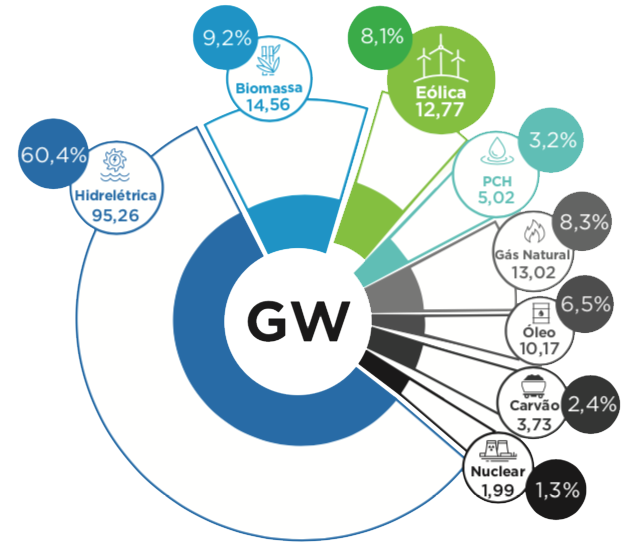
\includegraphics[width=0.75\linewidth]{./figuras/matriz-energetica-brasileira}
\caption{Matriz energética brasileira}
\label{Fig:matriz-energetica-brasileira}
\end{center} 
\end{figure}

Sendo um dos países que mais investe em energia eólica no mundo, o Brasil também é considerado um dos mais atrativos para investimentos em energias renováveis. A fonte eólica, sozinha, foi responsável por cerca de 80\% dos investimentos em renováveis no país de 2005 até 2015 \cite{CENARIO}. Um dos maiores motivos do alto investimento em energia eólica no Brasil é o alto valor do fator de capacidade proporcionado pelos ventos brasileiros. O fator de capacidade aponta o aproveitamento do vento para produção de energia e é representado pela proporção entre a geração efetiva da usina em um intervalo de tempo e a sua potência instalada. Em 2017 o valor médio do fator de capacidade no Brasil foi de 42,9\%, tendo atingido maior fator mensal médio em setembro, com 60,6\%, enquanto que no restante do mundo a média do é de 24,7\%.



O desempenho dos empreendimentos eólicos é fator determinante na definição do ritmo de crescimento e participação da fonte eólica na matriz elétrica brasileira e, consequentemente, no alcance das metas fixados pelo Governo.

O contributo social desta pesquisa é fornecer uma ferramenta que irá possibilitar o aumento da eficiência dos parques, conferindo, consequentemente, maior competitividade para a fonte eólica frente às demais fontes de geração, o que pode estimular a modicidade tarifária, a qual preconiza o consumo de energia mais barata para o cidadão brasileiro. Além disso, incentivar a expansão de fontes renováveis de energia, que não agridem o meio ambiente, é contribuir para o bem-estar humano.






Não há um número mínimo ou máximo de páginas para propostas de tema,
dissertações ou teses. Entretanto, se o seu documento for muito menor
do que a média pode transmitir uma ideia de falta de conteúdo a
apresentar. Por outro lado, um documento muito grande corre o risco de
só conseguir a atenção total do leitor no seu início, fazendo com que
as partes mais importantes, que geralmente estão no final do
documento, não sejam devidamente consideradas. Apenas para servir como
parâmetro, estão indicados a seguir os limites usuais quanto ao número
de páginas\footnote{Uma folha corresponde a uma página em impressão em
face simples e a duas páginas em impressão em face dupla} dos
documentos do PPgEEC da UFRN, adotando as margens e os espaçamentos
definidos neste modelo:
\begin{itemize}
\item Proposta de tema para exame de qualificação de mestrado:
entre 20 e 40 páginas
\item Proposta de tema para exame de qualificação de doutorado:
entre 30 e 50 páginas
\item Dissertação de mestrado:
entre 50 e 100 páginas
\item Tese de doutorado:
entre 80 e 150 páginas
\end{itemize}

O tamanho padrão para a fonte é de 12pt.  Para facilitar a escrita de
comentários, sugestões e correções da banca, recomenda-se o espaçamento
1.5 entre as linhas do texto e a impressão em um único lado da folhas
para os seguintes documentos:
\begin{itemize}
\item Proposta de tema para exame de qualificação;
\item Versão inicial de dissertação de mestrado; e
\item Versão inicial de tese de doutorado.
\end{itemize}
Para as versões finais de teses e dissertações, onde se busca uma
melhor qualidade visual e tipográfica do texto, deve-se utilizar
espaçamento simples entre as linhas e a impressão nos dois lados da
página.

As margens devem seguir os valores adotados neste documento, que podem
ser verificados no arquivo \texttt{principal.tex}. É importante notar
que, na versão final de teses ou dissertações, recomenda-se a
impressão nos dois lados da página. Por esta razão, a margem direita
em páginas pares deve ter o mesmo valor que a margem esquerda em
páginas impares e vice-versa, para que a encadernação fique
correta. Também em razão da impressão em frente e verso, os capítulos
devem sempre começar em uma página de número ímpar, com a eventual
inclusão de uma página em branco. O \LaTeX\ se encarrega de fazer
automaticamente estes ajustes.

\section{Robustez do sistema}
\label{RobustezSistema}

Documentos do porte de uma tese ou dissertação devem ser subdivididos
em capítulos. O capítulo deve conter uma introdução e um fecho.

A introdução do capítulo fornece ao leitor uma breve descrição do que
será tratado no capítulo e não forma uma seção: para exemplificar, a
introdução deste capítulo é o parágrafo que precede a primeira seção.

O fecho do capítulo apresenta comentários finais sobre o que foi
desenvolvido no capítulo e/ou faz uma ligação com o que será visto no
capítulo seguinte; normalmente é colo cado em uma seção específica,
denominada ``Comentários Finais'', ``Conclusões'', ``Resultados'',
``Avaliação Final'' ou qualquer outra denominação que se adéque ao
texto.

Capítulos são divididos em seções. O número ideal de seções é
impossível de se precisar. Entretanto, um capítulo com uma única seção
provavelmente deve ser agregado ao capítulo anterior ou posterior. Um
capítulo com quinze seções provavelmente deve ser subdividido em dois
capítulos.

Capítulos, seções e subseções devem ser rotulados para que possam ser
referenciados em qualquer parte do texto.  Isto é feito com o comando
\verb|\label{}|, que deve ser colocado logo após (nunca antes) o
comando que criou a seção, capítulo, etc. O parâmetro do comando
\texttt{label} é o nome simbólico que será usado para se fazer
referência a esta entidade dentro do texto, com o comando
\verb|\ref{}|. O nome pode ser qualquer coisa, mas não pode conter
acentos, por exemplo. Neste documento nós utilizamos a convenção de
prefixar os rótulos dos capítulos com \texttt{Cap:}, das seções com
\texttt{Sec:}, das equações com \texttt{Eq:} e assim por diante, mas
esta convenção não é obrigatória. Veja a seguir um exemplo de
utilização das referências cruzadas:
% quotation é um ambiente para citações, que ficam "recuadas" em
% relação ao resto do texto
\begin{quotation}
\dots no capítulo~\ref{Cap:Introducao} apresentamos um modelo de
capítulo de tese.
\end{quotation}
Note que, no código fonte deste trecho de frase, o espaço entre a palavra
\texttt{capítulo} e o comando \verb|\ref{}| foi escrito com
um \texttt{\~{}} e não com um espaço normal. O \texttt{\~{}} é o
comando \LaTeX\ para criar um espaço onde não se pode mudar de linha,
pois ficaria estranho se o texto ``no capítulo'' estivesse no fim de
uma linha e o número \ref{Cap:Introducao} no início da outra linha.

Existe uma particularidade no código fonte do parágrafo anterior. Para
se escrever:
\begin{quotation}
\dots o comando \LaTeX\ para criar\dots
\end{quotation}
se colocou depois do comando \verb|\LaTeX| um espaço
precedido de uma contrabarra, ao invés de um espaço normal. Isto porque
espaços depois de comandos são ignorados pelo \LaTeX; com um espaço
% Na linha anterior não houve necessidade do espaço com contrabarra
% depois do comando \LaTeX, pois ele é seguido por um ; e não um espaço
normal as palavras ficariam ligadas:
\begin{quotation}
\dots o comando \LaTeX para criar\dots
\end{quotation}
Ao invés do espaço precedido pela contrabarra, poder-se-ia também
utilizar um \texttt{\~{}}. A diferença é que neste caso o \LaTeX\ não
poderia fazer uma quebra de linha entre as palavras.
